\chapter{Software}\label{anx_sw}

\section{Gestor de paquetes opkg}\label{opkg}
Se puede configurar el gestor de paquetes de dos maneras para que encuentre los repositorios desde donde descargar los paquetes para su instalación. 

\bigskip
La primera de ellas es la más prolija y consiste en los siguientes pasos: 

\bigskip
Se crean los archivos xxx-feed.conf (xxx hace referencia a los subdirectorios dentro del repositorio) que contienen la ruta a los repositorios: 

\begin{verbatim}
$ echo src/gz angstrom-feed http://www.angstrom-
distribution.org/feeds/unstable/ipk/glibc/armv7a/base  
> /etc/opkg/angstrom-feed.conf 

$ echo src/gz perl-feed http://www.angstrom-distribution.
org/feeds/unstable/ipk/glibc/armv7a/perl/ 
> /etc/opkg/perl-feed.conf 

$ echo src/gz sdk-feed http://www.angstrom-distribution.
org/feeds/unstable/ipk/glibc/sdk/ > /etc/opkg/sdk-feed.conf 

$ echo src/gz python-feed http://www.angstrom-distribution.
org/feeds/unstable/ipk/glibc/armv7a/python/
> /etc/opkg/pyton-feed.conf 

$ echo src/gz debug-feed http://www.angstrom-distribution.
org/feeds/unstable/ipk/glibc/armv7a/debug/ 
> /etc/opkg/debug-feed.conf 

$ echo src/gz beagleboard-feed http://www.angstrom-
distribution.org/feeds/unstable/ipk/glibc/armv7a/machine/
beagleboard/ > /etc/opkg/beagleboard-feed.conf 

$ echo src/gz noarch-feed http://www.angstrom-distribution.
org/feeds/unstable/ipk/glibc/all/ > /etc/opkg/noarch-feed.
conf 
\end{verbatim}

Nota: /gz indica que los paquetes están comprimidos con extensión gz. 

\bigskip
Se debe actualizar la lista de paquetes disponibles:

\bigskip
\begin{verbatim}
$ opkg update
\end{verbatim}

El comando anterior crea los archivos /var/lib/opkg/xxx-feed que contienen la lista completa de paquetes en el repositorio. 

\bigskip
Nota: Se puede usar el comando opkg list $|$ wc -l para conocer la lista de paquetes. 

\bigskip
La segunda opción es modificar directamente el archivo /etc/opkg/opkg.conf a continuación de la línea: 

\bigskip
src $<$src-name$>$ $<$source-url$>$

\bigskip
Se agrega lo siguiente: 

\begin{verbatim}
src angstrom-feed http://www.angstrom-distribution.org/
feeds/unstable/ipk/glibc/armv7a/base/ 

src perl-feed http://www.angstrom-distribution.org/feeds/
unstable/ipk/glibc/armv7a/perl/ 

src sdk-feed http://www.angstrom-distribution.org/feeds/
unstable/ipk/glibc/sdk/ 

src python-feed http://www.angstrom-distribution.org/feeds/
unstable/ipk/glibc/armv7a/python/ 

src debug-feed http://www.angstrom-distribution.org/feeds/
unstable/ipk/glibc/armv7a/debug/ 

src beagleboard-feed http://www.angstrom-distribution.org/
feeds/unstable/ipk/glibc/armv7a/machine/beagleboard/ 

src noarch-feed http://www.angstrom-distribution.org/feeds/
unstable/ipk/glibc/all/ 
\end{verbatim}

Luego se actualiza la lista de paquetes:

\begin{verbatim}
$ opkg update
\end{verbatim}

Una vez que se agregan los repositorios es posible instalar paquetes mediante el comando: 

\begin{verbatim}
$ opkg install <nombre del paquete>
\end{verbatim}

El nombre del paquete puede buscarse en el sitio web que fue pasado como dirección del repositorio en la configuración anterior.

\bigskip
Por más información sobre le uso de este comando, referirse a \cite{AngManual} (ver apéndice \ref{HD}).

\section{Instalación, configuración y uso de SDK}\label{anx_sw_SDK}
Como fue comentado antes, el SDK es generado a partir de la herramienta web Narcissus. Para la instalación se debe tener el archivo (SDK.tar.bz2, por ejemplo) generado.

\bigskip
En el PC de desarrollo se debe hacer lo que sigue:

\bigskip
Se realiza la instalación con el usuario root y luego se explica como proceder con cualquier otro usuario.

\begin{verbatim}
$ sudo su
\end{verbatim}

Se descomprime el SDK en /

\begin{verbatim}
$ sudo tar -xf SDK.tar.bz2 -C /
\end{verbatim}

Se debe haber copiado el directorio angstrom en /usr/local

\bigskip
Luego, se habilita el uso del gestor de paquetes (opkg) y se agraga en el crosscompilador al PATH del sistema. Se debe establecer esta configuración con cada usuario que quiera utilizar la herramienta.

\begin{verbatim}
$ . /usr/local/angstrom/arm/environment-setup
\end{verbatim}

Lo que se tiene es un sistema Angström configurado en el PC de desarrollo con el que se puede actualizar la lista de repositorios, bajar paquetes, compilarlos para la arquitectura deseada, etc.

\bigskip
Actualización de repositorios:

\begin{verbatim}
$ opkg-target update
\end{verbatim}

Instalación de paquetes:

\begin{verbatim}
$ opkg-target install <paquete>
\end{verbatim}

Actualización de paquetes:

\begin{verbatim}
$ opkg-target upgrade
\end{verbatim}

El uso de opkg-target es solo permitido para el usuario root por un tema de permisos, aunque el uso del crosscompilador es permitido para cualquier usuario siempre y cuando haga lo siguiente cada vez que vaya a utilizar la herramienta:

\begin{verbatim}
$ . /usr/local/angstrom/arm/environment-setup
\end{verbatim}

Para referirse a las herramientas de la arquitectura para la cual se generan los binarios se utiliza el prefijo arm-angstrom-linux-gnueabi-.

\bigskip
Por más detalles referirse a \cite{conf_SDK}.


\section{OpenEmbedded-Bitbake}\label{anx_sw_oe}

Para la instalación, configuración y ejecución de esta herramienta, se deben seguir los pasos en detalle. Se debe tener una buena conexión a internet para la descarga de fuentes, espacio libre en disco duro de no menos de 10GB, buen procesador y paciencia ya que los desarrollos completos demoran varias horas.

\bigskip
Primero se instalan los paquetes previos necesarios. 

\newpage
Paquetes importantes:

\begin{verbatim}
$ sudo apt-get install sed wget cvs subversion git-core \

coreutils unzip texi2html texinfo docbook-utils \

gawk python-pysqlite2 diffstat help2man make gcc \

build-essential g++ desktop-file-utils chrpath
\end{verbatim}

Paquetes secundarios (aceleran los procesos):

\begin{verbatim}
$ sudo apt-get install libxml2-utils xmlto python-psyco apr
\end{verbatim}

Chequear que /bin/sh no tiene un enlace simbólico a “dash”:

\begin{verbatim}
$ ls -l /bin/sh
\end{verbatim}

Debe estar enlazado a “bash”. Si no lo está:

\begin{verbatim}
$ sudo dpkg-reconfigure dash
\end{verbatim}

Aquí seleccionamos NO instalar “dash” como /bin/sh

\bigskip
Compilador para aumentar la velocidad de bitbake:

\begin{verbatim}
$ sudo apt-get install python-psyco
\end{verbatim}

Para versiones de Ubuntu mayores o iguales a la 10.04:

\begin{verbatim}
$ sudo su

$ echo 128 > /proc/sys/vm/mmap_min_addr

$ exit

$ sudo sysctl -w vm.mmap_min_addr=128
\end{verbatim}

\leftline{Instalación:}

\bigskip
El directorio base seleccionado para el desarrollo con OpenEmbedded es stuff (puede ser otro), y se ubicó en /.

\bigskip
Se crea la estructura de directorios:

\begin{verbatim}
$ sudo mkdir -p /stuff/build/conf

$ cd /stuff/
\end{verbatim}

Bitbake es la herramienta de construcción que utiliza OpenEmbedded. Está escrita en Python, por lo que no es necesario compilarlo para que funcione.

\begin{verbatim}
$ sudo wget http://download.berlios.de/bitbake/
bitbake-1.10.2.tar.gz
\end{verbatim}

Nota: esta es la última versión disponible al momento. Para saber cual es la última versión disponible, entrar a: http://download.berlios.de/bitbake/.

Para las nuevas versiones es necesario tener instalado Python 2.6 o posterior.

\bigskip
Luego se descomprime el tar.gz bajado:

\begin{verbatim}
$ sudo tar -xzf bitbake-1.10.2.tar.gz

$ ls
\end{verbatim}

Se debe ver un directorio llamado en este caso bitbake-1.10.2 (se puede renombrar a: “bitbake” por comodidad).

\bigskip
Para obtener OpenEmbedded es necesario tener instalado git.

\bigskip
Ahora se hace lo siguiente:

\begin{verbatim}
$ cd /stuff

$ sudo git clone git://git.openembedded.org/openembedded
\end{verbatim}

Nota: git clone es para hacer un checkout del repositorio. 

Otro repositorio es http://repo.or.cz/r/openembedded.git

\bigskip
Demora mucho. Al finalizar se crea un directorio con el nombre openembedded.

\bigskip
Se recomienda actualizar OpenEmbedded una vez al día:

\begin{verbatim}
$ cd /stuff/openembedded

$ sudo git pull
\end{verbatim}

\newpage
\leftline{Configuración:}

\bigskip
Se modifica la configuración local, donde se debe indicar todo lo que se quiera crear.

\begin{verbatim}
$ cd /stuff/

$ sudo cp openembedded/conf/local.conf.sample build/conf/
local.conf

$ sudo vi build/conf/local.conf
\end{verbatim}

Nota: en lugar de vi, se pueden usar nano o incluso gedit. Estos son editores de texto ordenados por complejidad.

\bigskip
En este punto hay que tener cuidado debido a que existen muchas variables a editar y se necesita mucho conocimiento para poder cambiarlas.


La mínima cantidad de variables a editar para un desarrollo correcto son las siguientes:

\bigskip
BBFILES = “/stuff/openembedded/recipes/*/*.bb”

MACHINE = “beagleboard”

DISTRO = “angstrom-2008.1”

PARALLEL\_MAKE = “-j 5”

INHERIT += “rm\_work”

\bigskip
Nota: Los parámetros detallados antes ya existen en el archivo de configuración, algunos deben ser descomentados y/o editados ya que lo único que cambia es el valor asignado.

\bigskip
BBFILES: indica que archivos son considerados durante el desarrollo.

\bigskip
MACHINE: el nombre asociado a la SBC que se esté usando. Para saber el nombre asociado a la SBC se puede ver el contenido del directorio

\leftline{/stuff/openembedded/conf/machine.}

\bigskip
DISTRO: qué versión de la distribución se quiere instalar. Aquí se eligió la última versión estable de Angström, aunque si se pone “angstrom-2010.x”, se obtiene una versión más nueva (no asegura estabilidad). La versión no solo afecta a la distribución sino que la versión del kernel generado va a depender de esta versión. Por ejemplo, con 2008.1 se obtiene un kernel 2.6.32 y con 2010.x se obtiene un kernel 2.6.37. Para saber cuales son las versiones disponibles al momento se puede ver el contenido del directorio 
/stuff/openembedded/conf/distro.

\bigskip
PARALLEL\_MAKE: indica cuantas operaciones simultáneas puede realizar el procesador de la pc de desarrollo. En general el valor se puede calcular como sigue: (cantidad de procesadores)x2 +1. En este caso 5 equivale a una cpu del tipo core2duo.

\bigskip
INHERIT += “rm\_work”: esta opción elimina los fuentes después de haber construido los paquetes. Esto hace que el tamaño del desarrollo en disco, no supere los 10 GB. Si esta opción no se elige, se deben tener por lo menos 40 GB de espacio libre en disco duro. También se puede decir que si se elige esta opción algunos fuentes deberán ser bajados nuevamente en cada desarrollo, lo que lo puede hacer más lento.


\bigskip
Conviene leer todo el archivo para tener una idea básica de lo que hace. Si en algún lugar se quiere hacer referencia al “home” del usuario, la ruta se debe escribir completa (no se puede $\sim$).

La última línea debe ser borrada (esto es para asegurarse de que se leyó todo). 

\bigskip
\leftline{Ejecución:}

\bigskip
Siempre antes de empezar a desarrollar se debe ejecutar lo siguiente:

\begin{verbatim}
$ export BBPATH=/stuff/build:/stuff/openembedded

$ export PATH=/stuff/bitbake/bin:$PATH
\end{verbatim}

Comenzando el desarrollo:

\begin{verbatim}
$ cd /stuff/build

$ bitbake console-image
\end{verbatim}

Nota: Al ejecutarlo por primera vez, demora varias horas. 

\bigskip
Si aparecen errores como “Please set persistent and cache” o “no se puede acceder al directorio tmp” esto se soluciona dando permisos al directorio stuff:

\begin{verbatim}
$ sudo su

$ chmod -R 777 /stuff
\end{verbatim}

El comando bitbake console-image baja todos los fuentes y genera todos los binarios necesarios para la ejecución de la  distribución Angström en modo consola. Otra opción, si solo queremos un kernel, es el comando bitbake virtual/kernel, pero para entender bien el funcionamiento del bitbake, la primera vez se recomienda bitbake console-image.

\bigskip
Luego de ejecutado el comando, se crea toda la estructura de directorios.

\bigskip
A continuación se detallan los más importantes:

\bigskip
/stuff/build/tmp/deploy/glibc/images/beagleboard/ 

Aquí se guardan los archivos generados.

\bigskip
/stuff/build/tmp/work/beagleboard-angstrom-linux-gnueabi/

Aquí se encuentran los directorios con los fuentes del kernel y el u-boot.

\section{u-boot}\label{anx_sw_ub}

Nota: Puede que cuando se realiza la instalación de OpenEmbedded-Bitbake, se genere un directorio relacionado con u-boot en /stuff/build/tmp/work/beagleboard-angstrom-linux-gnueabi/, si esto es así, no es necesario volver a obtener los fuentes.

\bigskip
\leftline{Se configura el bitbake para poder utilizarlo:}

\bigskip
\begin{verbatim}
$ export BBPATH=/stuff/build:/stuff/openembedded

$ export PATH=/stuff/bitbake/bin:$PATH
\end{verbatim}

\bigskip
\leftline{Se obtienen los fuentes:}

\begin{verbatim}
$ cd /stuff/build

$ bitbake -f -c clean -b ../openembedded/recipes/u-boot/
u-boot_git.bb

$ bitbake -f -c compile -b ../openembedded/recipes/u-boot/
u-boot_git.bb
\end{verbatim}

\bigskip
Los fuentes se encuentran en 

/stuff/build/tmp/work/beagleboard-angstrom-linux-gnueabi/u-boot.../git/.

\bigskip
En los fuentes del u-boot dentro de board/ti/beagle/ se encuentra el archivo beagle.h que es donde se establece la configuración de los pines del bloque de expansión de la Beagleboard.

Si se abre este archivo se ven líneas del estilo: 

\begin{verbatim}
MUX_VAL(CP(MCBSP3_DX), (IEN | PTD | DIS | M4)) /*GPIO_140*/\
\end{verbatim}

MUX\_VAL indica que se va a modificar el valor de multiplexado de lo que está entre paréntesis. 

\bigskip
CP(MCBSP3\_DX) es el Control\_PadConf, esto es el registro del microprocesador asociado con el 
pin a modificar. 

\bigskip
(IEN $|$ PTD $|$ DIS $|$ M4) es la configuración del pin en cuestión: 


La opción IEN (input enable) hace que el pin sea bidireccional. 

La opción PTD y PTU, indica si el pin tiene un pull down o pull up respectivamente. 

La opción DIS y EN, indica si se deshabilitan o no las opciones PTD y PTU respectivamente. 

La opción M4 es el modo seleccionado para el pin. Para la Beagleboard existen cuatro modos: M1, M2, M3 y M4.

\bigskip
GPIO\_140 es el nombre del pin (solo es un comentario). 

\bigskip
El Control\_PadConf es un registro de 32bits que controla el estado de dos pines, esto es, la parte 
baja del registro controla un pin y la parte alta controla otro. 

Analizando el “manual de referencia Beagleboard del usuario” (“Expansion connector signals” – tabla 20), y “manual técnico de referencia OMAP35x” (“SCM functional description” – capítulo 7.4.4); ambos adjuntos en el apéndice \ref{HD}; y agregando las opciones que interesan para los pines, se confeccionó la siguiente tabla: 

\newpage
\begin{longtable}{|c|p{2.6cm}|c|p{2.5cm}|c|}
\hline
\textbf{CONTROL\_PADCONF\_} & \textbf{EQUIV. BEAGLE.H} & \textbf{PIN EXPANSIÓN} & \textbf{SEÑAL EN EL PIN} & \textbf{MODO} \\ \hline
MMC2\_DAT6[31:16] & MMC2\_DAT7 & 3 & GPIO\_139 & 4 \\ \hline
UART2\_CTS[15:0] & UART2\_CTS & 4 & GPIO\_144 & 4 \\ \hline
MMC2\_DAT6[15:0] & MMC2\_DAT6 & 5 & GPIO\_138 & 4 \\ \hline
UART2\_TX[15:0] & UART2\_TX & 6 & UART2\_TX & 0 \\ \hline
MMC2\_DAT4[31:16] & MMC2\_DAT5 & 7 & GPIO\_137 & 4 \\ \hline
McBSP3\_CLKX[31:16] & McBSP3\_FSX & 8 & UART2\_RX & 1 \\ \hline
MMC2\_DAT4[15:0] & MMC2\_DAT4 & 9 & GPIO\_136 & 4 \\ \hline
UART2\_CTS[31:16] & UART2\_RTS & 10 & GPIO\_145 & 4 \\ \hline
MMC2\_DAT2[31:16] & MMC2\_DAT3 & 11 & McSPI3\_CS0 & 1 \\ \hline
McBSP1\_DX[15:0] & McBSP1\_DX & 12 & GPIO\_158 & 4 \\ \hline
MMC2\_DAT2[15:0] & MMC2\_DAT2 & 13 & GPIO\_134 & 4 \\ \hline
McBSP1\_CLKX[15:0] & McBSP1\_CLKX & 14 & GPIO\_162 & 4 \\ \hline
MMC2\_DAT0[31:16] & MMC2\_DAT1 & 15 & GPIO\_133 & 4 \\ \hline
McBSP\_CLKS[31:16] & McBSP1\_FSX & 16 & GPIO\_161 & 4 \\ \hline
MMC2\_DAT0[15:0] & MMC2\_DAT0 & 17 & McSPI3\_SOMI & 1 \\ \hline
McBSP1\_DX[31:16] & McBSP1\_DR & 18 & GPIO\_159 & 4 \\ \hline
MMC2\_CLK[31:16] & MMC2\_CMD & 19 & McSPI3\_SIMO & 1 \\ \hline
McBSP1\_CLKR[15:0] & McBSP1\_CLKR & 20 & GPIO\_156 & 4 \\ \hline
MMC2\_CLK[15:0] & MMC2\_CLK & 21 & McSPI3\_CLK & 1 \\ \hline
McBSP1\_CLKR[31:16] & McBSP1\_FSR & 22 & GPIO\_157 & 4 \\ \hline
I2C2\_SDA[15:0] & I2C2\_SDA & 23 & GPIO\_183 & 4 \\ \hline
I2C1\_SDA[31:16] & I2C2\_SCL & 24 & GPIO\_168 & 4 \\ \hline
\caption{Modo de pines en bloque de expansión}\label{pines}
\end{longtable}

Al modificar el archivo beagle.h hay que tener mucho cuidado, ya que al sustituir los valores no se deben repetir pines ni registros, no deben haber incoherencias, un registro por cada pin y un pin por cada registro. 
Dentro del archivo hay un macro definido MUX\_BEAGLE\_C(), donde se deben realizar las modificaciones ya que este macro está asociado con el modelo de Beagleboard utilizado (C4).\\
En una primera instancia se sustituyeron los valores del cuadro \ref{pines} buscando los equivalentes del 
PadConf en el archivo beagle.h. 


\begin{verbatim}
\#define MUX_BEAGLE_C() \
MUX_VAL(CP(MCBSP3_DX),   (IEN  | PTD | DIS | M4))/*GPIO_140*/\
MUX_VAL(CP(MCBSP3_DR),   (IEN  | PTD | DIS | M4))/*GPIO_142*/\
MUX_VAL(CP(MCBSP3_CLKX), (IEN  | PTD | DIS | M4))/*GPIO_141*/\
MUX_VAL(CP(MCBSP3_FSX),  (IEN  | PTD | DIS | M1))/*UART2_RX*/\
MUX_VAL(CP(UART2_TX),    (IDIS | PTD | DIS | M0))/*UART2_TX*/\
MUX_VAL(CP(MMC2_DAT7),   (IEN  | PTD | EN  | M4))/*GPIO_139*/\
MUX_VAL(CP(UART2_CTS),   (IEN  | PTD | DIS | M4))/*GPIO_144*/\
MUX_VAL(CP(MMC2_DAT6),   (IEN  | PTD | EN  | M4))/*GPIO_138*/\
MUX_VAL(CP(MMC2_DAT5),   (IEN  | PTD | EN  | M4))/*GPIO_137*/\
MUX_VAL(CP(MMC2_DAT4),   (IEN  | PTD | EN  | M4))/*GPIO_136*/\
MUX_VAL(CP(UART2_RTS),   (IEN  | PTD | EN  | M4))/*GPIO_145*/\
MUX_VAL(CP(MCBSP1_DX),   (IEN  | PTD | EN  | M4))/*GPIO_158*/\
MUX_VAL(CP(MMC2_DAT2),   (IEN  | PTD | EN  | M4))/*GPIO_134*/\
MUX_VAL(CP(MCBSP1_CLKX), (IEN  | PTD | EN  | M4))/*GPIO_162*/\
MUX_VAL(CP(MMC2_DAT1),   (IEN  | PTU | EN  | M4))/*GPIO_133*/\
MUX_VAL(CP(MCBSP1_FSX),  (IEN  | PTD | EN  | M4))/*GPIO_161*/\
MUX_VAL(CP(MCBSP1_DR),   (IEN  | PTD | EN  | M4))/*GPIO_159*/\
MUX_VAL(CP(MCBSP1_CLKR), (IEN  | PTD | EN  | M4))/*GPIO_156*/\
MUX_VAL(CP(MCBSP1_FSR),  (IEN  | PTD | EN  | M4))/*GPIO_157*/\
MUX_VAL(CP(I2C2_SDA),    (IEN  | PTD | EN  | M4))/*GPIO_183*/\
MUX_VAL(CP(I2C2_SCL),    (IEN  | PTU | EN  | M4))/*GPIO_168*/\
MUX_VAL(CP(MMC2_DAT3),   (IEN  | PTD | EN  | M1))/*SPI3_CS0*/\
MUX_VAL(CP(MMC2_DAT0),   (IEN  | PTU | EN  | M1))/*SPI3_SOMI*/\
MUX_VAL(CP(MMC2_CMD),    (IEN  | PTU | DIS | M1))/*SPI3_SIMO*/\
MUX_VAL(CP(MMC2_CLK),    (IEN  | PTU | DIS | M1))/*SPI3_CLK*/
\end{verbatim}

Luego es necesario compilar para obtener el u-boot.bin.

\bigskip
\begin{verbatim}
$ cd /stuff/build

$ bitbake -f -c compile -b ../openembedded/recipes/u-boot/
u-boot_git.bb

$ bitbake -f -c deploy -b ../openembedded/recipes/u-boot/
u-boot_git.bb
\end{verbatim}

\bigskip
Nota: Cada vez que se introduzca un nuevo cambio, no es necesario ejecutar el comando con la opción clean (lo que implica volver a bajar los fuentes), solo basta con volver a compilar.


\section{uImage}\label{ker}

A continuación se detallan los pasos a seguir para la modificación de los fuentes del kernel:
 
\bigskip
Comando necesario para el desarrollo del uImage:

\begin{verbatim}
$ bitbake virtual/kernel -c [comando]
\end{verbatim}

virtual/kernel: refiere a que se quiere generar un kernel.

\bigskip
Entre los comandos:

\bigskip
clean: borra el contenido del directorio work. Borra todos los cambios hechos en la configuración del uImage fuente y parches agregados.

patch: genera los archivos de configuración y el fuente del uImage. Además le aplica los parches.

menuconfig: abre el editor de la configuración del kernel.

compile: compila todo.

deploy: genera los archivos referidos en este caso al uImage (.config, módulos, uImage) y los guarda en el directorio /stuff/build/tmp/deploy/glibc/images/beagleboard/.

\bigskip
Nota: Es necesario que todos estos comandos sean ejecutados en el orden adecuado para que todo funcione correctamente.

\bigskip
Primero se configura bitbake para poder utilizarlo:

\begin{verbatim}
$ export BBPATH=/stuff/build:/stuff/openembedded

$ export PATH=/stuff/bitbake/bin:$PATH
\end{verbatim}

\bigskip
Se comienza el desarrollo:

\begin{verbatim}
$ cd /stuff/build

$ bitbake virtual/kernel -c clean

$ bitbake virtual/kernel -c patch

$ bitbake virtual/kernel -c menuconfig
\end{verbatim}

\bigskip
Luego de ejecutar este comando se abre el editor de la configuración del kernel (ver figura \ref{Fig:kernel}). Este editor especifica qué componentes compilar, y si la imagen generada incluye el componente de forma estática o modular. En este caso un cambio de  configuración es necesario para el buen funcionamiento de la interfaz SPI y de la conexión USB-ethernet con la Beagleboard.

\begin{figure}[H]
\centering
  \begin{center}
  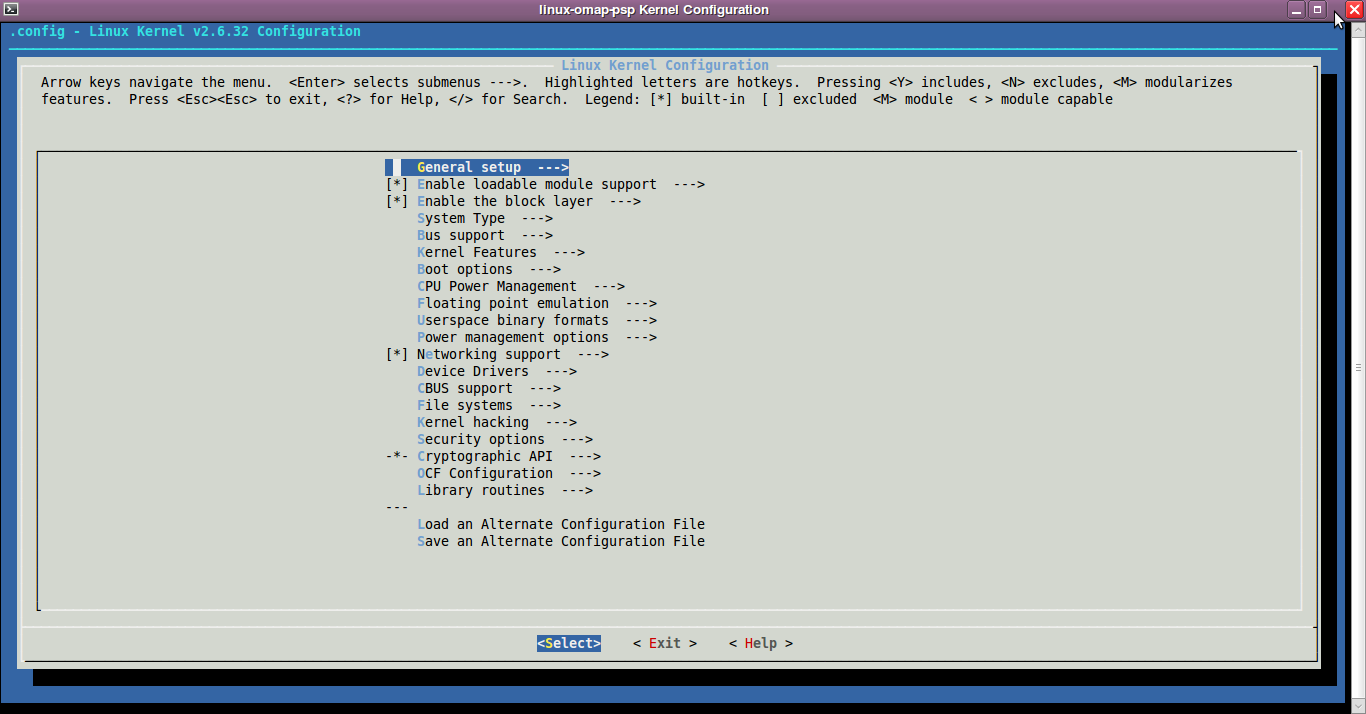
\includegraphics[scale=.3]{Imagenes/kernel.png} 
  \end{center}
  \caption{Editor de configuración del kernel}\label{Fig:kernel} 
\end{figure}

Para configurar la interfaz SPI, se debe configurar como sigue:

Device Drivers – SPI Support=y y luego como en la figura \ref{Fig:spi}.

\begin{figure}[H]
\centering
  \begin{center}
  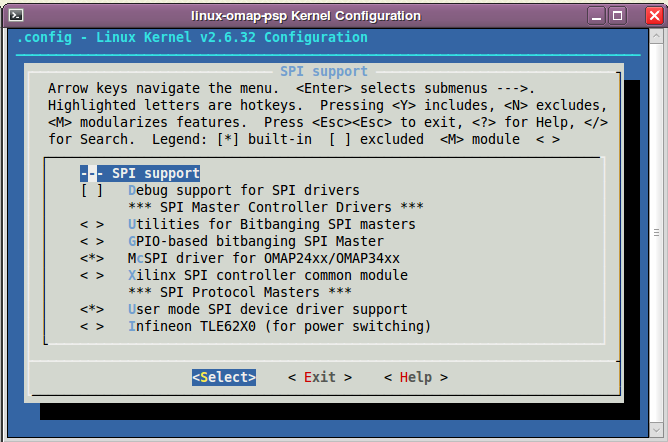
\includegraphics[scale=.4]{Imagenes/spi_chica.png} 
  \end{center}
  \caption{Configuración SPI}\label{Fig:spi} 
\end{figure}

\newpage
Para poder establecer la conexión por USB con la Beagleboard, se debe configurar como sigue: 

Device Drivers – USB Support=y – USB Gadget Support=y y luego como en la figura \ref{Fig:usb}.

\begin{figure}[H]
\centering
  \begin{center}
  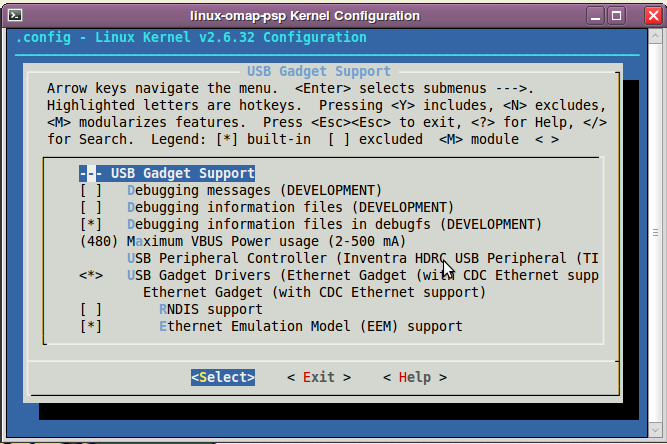
\includegraphics[scale=.4]{Imagenes/usb_chica.png} 
  \end{center}
  \caption{Configuración USB Gadget}\label{Fig:usb} 
\end{figure}

Luego, es necesario modificar el archivo board\_omap3beagle.c que se encuentra en /stuff/build/tmp/work/beagleboard-angstrom-linux-gnueabi/linux-omap-.../git/arch/arm/
mach-omap2/. En este archivo está toda la inicialización de las interfaces. Los detalles de los cambios introducidos en este archivo se pueden observar en el apéndice \ref{anx_sw_uIm}.

\bigskip
Se compila y genera el archivo uImage:

\bigskip
\begin{verbatim}
$ bitbake virtual/kernel -c compile

$ bitbake virtual/kernel -c deploy
\end{verbatim}

\bigskip
Dentro de /stuff/build/tmp/deploy/glibc/images/beagleboard/ se encuentra el archivo uImage generado.

\bigskip
Nota: Respecto al nombre del archivo, al igual que con el caso del u-boot.bin el nombre que aparece es un nombre más largo y necesita ser renombrado a uImage para que se pueda ejecutar correctamente.

\subsection{Cambios introducidos en el archivo board\_omap3beagle.c}\label{anx_sw_uIm}

Se detallan las modificaciones en el archivo board\_omap3beagle.c necesarios para la inicialización correcta de las interfaces SPI y GPIO. Como ya se comentó este archivo está ubicado en /stuff/build/tmp/work/beagleboard-angstrom-linux-gnueabi/linux-omap-.../git/arch/arm/mach-omap2/ y es el encargado de toda la inicialización de las interfaces del sistema.

\bigskip
En el caso de la interfaz SPI se vio que no se lograba un mapeo de la interfaz en /dev, lo que no permitía el acceso a ésta a nivel de usuario. En el caso de la interfaz GPIO se vio que para los pines GPIO no basta con los cambios realizados en el u-boot para establecer su dirección y valor al iniciar el sistema.
A continuación se plantea una posible solución para ambos casos.

\bigskip
\leftline{Cambios asociados al SPI:}

\bigskip
Se creó una estructura (spi\_board\_info beagle\_mcspi\_board\_info) que contempla todas las posibilidades de interfaz SPI en la Beagleboard y agrega información sobre éstas.
En la estrucutra se pueden ver tres formas de representar al SPI: spi3.0, spi3.1 y spi4.0. El microprocesador de la Beagleboard tiene 4 interfaces SPI disponibles de las cuales la 3 y la 4 son accesibles desde el bloque de expansión de la Beagleboard. Además la interfaz spi3 se puede encontrar en dos modalidades 3.0 o 3.1 dependiendo de si se utiliza el CS0 o el CS1 como chip select de la interfaz. La interfaz spi4 solo puede utilizar el CS0.
Es por esto que en la estructura se definen spi3.0, spi3.1 y spi4.0.
Dentro de cada interfaz definida se agrega información sobre la interfaz, como ser el nombre (modalias), la máxima velocidad de transferencia/recepción de datos (max\_speed\_hz), número de bus (bus\_num), chip select (chip\_select) y modo del spi (SPI\_MODE\_1).

\begin{verbatim}
static struct spi_board_info beagle_mcspi_board_info[] = { 
    /* spi 3.0 */ 
    { 
        .modalias	= "spidev", 
        .max_speed_hz	= 48000000, /* 48 Mbps */ 
        .bus_num	= 3, 
        .chip_select	= 0,	 
        .mode = SPI_MODE_1, 
    }, 
    /* spi 3.1 */ 
    { 
        .modalias	= "spidev", 
        .max_speed_hz	= 48000000, /* 48 Mbps */ 
        .bus_num	= 3, 
        .chip_select	= 1,	 
        .mode = SPI_MODE_1, 
    }, 
    /* spi 4.0 */ 
    { 
        .modalias	= "spidev", 
        .max_speed_hz	= 48000000, /* 48 Mbps */ 
        .bus_num	= 4, 
        .chip_select	= 0,	 
        .mode = SPI_MODE_1, 
    }, 
 }; 
\end{verbatim}

\newpage
Luego de definidas las interfaces fue creada una función (omap3\_beagle\_init\_spi\_rf2) que las inicializara.

\begin{verbatim}
static void __init omap3_beagle_init_spi_rf2(void) 
{ 
    printk(KERN_INFO "Usando SPI\n");  
    /* hook the spi ports to the spidev driver */ 
    spi_register_board_info(beagle_mcspi_board_info, 
    ARRAY_SIZE(beagle_mcspi_board_info)); 
}
\end{verbatim}

Para que la función de inicialización de la interfaz SPI pueda ejecutarse, se debe hacer referencia a ésta en la función general de inicialización de interfaces asociada a la Beagleboard (omap3\_beagle\_init).

\begin{verbatim}
omap3_beagle_init_spi_rf2();
\end{verbatim}

Con estos cambios se logró que las interfaces SPI sean accesibles en el espacio de usuario bajo /dev y mapeadas como spidev3.0, spidev3.1, spidev4.0.

\bigskip
\leftline{Cambios asociados al GPIO:}

\bigskip
Se creó una función (gpio\_config\_rf2) que dado un número asociado con el pin GPIO, establece su dirección y valor.

\begin{verbatim}
static void gpio_config_rf2(unsigned gpio, int direction, 
int value) {
  /* Tell the kernel, we want to use the GPIO*/
  if (gpio_request(gpio, "gpio\n") != 0) {
    printk(KERN_ALERT "Unable to request GPIO %d\n", 
    gpio);
  }
  else {
    /* Now tell the kernel that GPIO is an (in-out)put 
    and should be set to value (only as output) */
    switch (direction) {
      case 0: if (gpio_direction_output(gpio, value) != 0) {
                printk(KERN_ALERT "Unable to set GPIO 
                direction for GPIO %d\n", gpio);
              }
              else {
                /* enable direction on userspace */
                if (gpio_export(gpio, 1) != 0){ 
                  printk(KERN_ALERT "Unable to set GPIO 
                  export for GPIO %d\n", gpio);
                }
              }
              break;
      case 1: if (gpio_direction_input(gpio) != 0) {
                printk(KERN_ALERT "Unable to set GPIO 
                direction for GPIO %d\n", gpio);
              }
              else {
                /* enable direction on userspace */
                if (gpio_export(gpio, 1) != 0) { 
                  printk(KERN_ALERT "Unable to set GPIO 
                  export for GPIO %d\n", gpio);
                }
              }
              break;
      default: break;
    }
  }	
}
\end{verbatim}

Se creó la función de inicialización (gpio\_rf2) que establece la configuración de todos los pines GPIO del sistema RF$^{2}$.

\begin{verbatim}
static void __init gpio_rf2(void)
{
    printk(KERN_ALERT "Configurando GPIO RF2...\n");
    gpio_config_rf2(133, 0, 1); /*E*/
    gpio_config_rf2(134, 0, 0); /*D5*/
    gpio_config_rf2(136, 0, 0); /*D7*/
    gpio_config_rf2(137, 0, 0); /*XOE*/
    gpio_config_rf2(138, 0, 0); /*led rojo*/
    gpio_config_rf2(139, 0, 0); /*led_verde*/
    gpio_config_rf2(144, 0, 0); /*RST_SC*/
    gpio_config_rf2(145, 0, 0); /*led_amarillo*/
    gpio_config_rf2(156, 0, 0); /*RW*/
    gpio_config_rf2(157, 0, 0); /*RS*/
    gpio_config_rf2(158, 0, 0); /*Buzzer*/
    gpio_config_rf2(159, 0, 0); /*D4*/
    gpio_config_rf2(161, 0, 0); /*D6*/
    gpio_config_rf2(162, 0, 0); /*Backlight*/
    gpio_config_rf2(168, 0, 1); /*RST_RF*/
    gpio_config_rf2(183, 1, 0); /*IRQ_RF*/
}
\end{verbatim}

Luego, como en el caso de la interfaz SPI, se debe hacer referencia a la función anterior en la función de inicialización del sistema (omap3\_beagle\_init).

\begin{verbatim}
gpio_rf2();
\end{verbatim}

Con estos cambios se logró una cambio en la configuración de los pines GPIO, según la dirección y el valor que les corresponde para el buen funcionamiento del sistema RF$^{2}$.

\section{FileSystem}\label{narc}

A continuación se detallan las diferentes características y opciones que se eligieron para crear un fileSystem a medida para la Beagleboard y un SDK para el PC de desarrollo:

\bigskip
Select Machine: Beagleboard.

\bigskip
Image Name: el nombre que se le quiera dar.

\bigskip
Complexity: complejidad, se eligió “advanced” ya que la opción “simple” no brinda libertad de configuración.

\bigskip
Release: versión, aquí hay varias opciones disponibles, se eligió “unstable” ya que es la más estable de las disponibles. La primera opción disponible es la más estable.

\bigskip
Base System: aquí se elige el soporte de drivers y paquetes que se pretenden. “bare bones” es la opción con menos soporte y “extended” es la de mayor soporte. Cuanto más soporte, más pesado se hace el fileSystem. Una opción interesante es la opción “regular”, y es la que se eligió.

\bigskip
/dev manager: esto es el manejador de /dev, se recomienda “udev”.

\bigskip
Type of Image: formato en el que se quiere descargar el fileSystem. Se eligió “tar.gz” ya que es la opción más versátil.

\bigskip
Software manifest: se genera un archivo en la web con todos los paquetes que se instalaron en detalle.

\bigskip
SDK type: esta opción permite generar un SDK para el PC de desarrollo compatible con el fileSystem generado. Esto es sumamente útil por ejemplo para crosscompilar. Aquí se eligió la opción “Full SDK”.

\bigskip
User environment section: aquí se indica que tipo de sistema operativo se quiere, básicamente se tienen dos opciones; una es un fileSystem sin interfaz gráfica y las otra con entorno gráfico. Se eligió la opción “console” (sin entorno gráfico) ya que la aplicación no exige entorno gráfico.

\bigskip
Luego se permite seleccionar programas que se desean instalar.
Las aplicaciones elegidas son: nano editor (editor de texto) ya que hace las cosas más fáciles que el programa vi, GDB y GDBServer necesarios para la depuración de la aplicación, y toolchain para tener herramientas de compilación nativas en la Beagleboard.

\bigskip
Cuando todo fue seleccionado, se da un click en “build me” (demora un poco).
Cuando el proceso termina, se generan dos archivos comprimidos, un archivo con el nombre elegido para la imagen en un formato .tar.gz y el SDK para el PC de desarrollo en formato .tar.bz2. 


\section{Instalación y configuración de librfid-tool}\label{ins_conf_librfid}

A continiuación se detalla la instalación y configuración de librfid para su uso con OpenPCD y con el lector/escritor RFID diseñado.

\bigskip
Para comenzar se descarga la biblioteca:

\begin{verbatim}
$ svn checkout https://svn.gnumonks.org/trunk/librfid/
\end{verbatim}

Dentro del directorio raíz, se encuentran una serie de directorios con los fuentes. Los más importantes se detallan a continuación:

\bigskip
utils: en este directorio de encuentran las funciones asociadas con la herramienta librfid-tool. Se destaca librfid-tool.c donde se encuentra la función main de la aplicación librfid-tool.

\bigskip
src: en este directorio se encuentran todos los fuentes de la biblioteca librfid.

\bigskip
include: en este directorio se encuentran todos los encabezados de las funciones de la biblioteca librfid.


\bigskip
\leftline{OpenPCD}

\bigskip
Para comenzar se intentó la comunicación desde el PC para luego pasar a la Beagleboard, ya que existe mucha documentación para el primer caso [REF]. En los dos casos fue necesario compilar la biblioteca para utilizar en la arquitectura elegida.

\bigskip
OpenPCD en PC:

\bigskip
Como primer paso, se conecta el OpenPCD al PC. Para saber si el dispositivo es detectado por la PC, es necesario lo siguiente:

\begin{verbatim}
$ lsusb
\end{verbatim}

Aquí debe aparecer (entre otros dispositivos conectados) un dispositivo con un identificador ID 16c0:076b (vendor:product). 

\bigskip
Nota: En caso de que este dispositivo no aparezca, se debe usar un HUB con alimentación externa.

\bigskip
Compilando librfid:

\bigskip
Para compilar la biblioteca son necesarios los siguientes paquetes: libtool, libusb-dev, libcurl-dev (libcurl4gnutls-dev instalado en este caso).

\bigskip
Se debe ir hasta el directorio donde se encuentra la biblioteca descargada (librfid por ejemplo) y escribir lo siguiente:

\begin{verbatim}
$ cd librfid

$ ./configure

$ make

$ sudo make install
\end{verbatim}

OpenPCD en la Beagleboard:

\bigskip
Antes que nada se debe conectar el OpenPCD a la Beagleboard y verificar que es detectado al igual que en la instalación en el PC:

\begin{verbatim}
$ lsusb
\end{verbatim}

Se tuvo que utilizar un HUB con alimentación externa ya que la Beagleboard no logró ver al OpenPCD.

\bigskip
La compilación se realiza directamente en la Beagleboard.

\bigskip
Al igual que en el caso de la compilación para el uso en un PC, se debieron obtener los paquetes libtool, libusb-dev, libcurl-dev. Para instalar los paquetes se utilizó el siguiente comando:

\begin{verbatim}
$ opkg install “paquete”
\end{verbatim} 

Se copia la biblioteca (sin compilar) a la Beagleboard y luego:

\begin{verbatim}
$ cd librfid

$ ./configure

$ make

$ make install
\end{verbatim}


Lector-escritor RFID en la Beagleboard:

\bigskip
El lector/escritor RFID se conecta a la Beagleboard a través de una interfaz SPI.
Para habilitar las funcionalidades de la librfid asociadas con la comunicación SPI, es necesario indicar al configurar, que se quiere utilizar esta interfaz a través de la opción $--$enable-spidev. La compilación se realiza en la Beagleboard:

\begin{verbatim}
$ cd librfid

$ ./configure --enable-spidev

$ make

$ make install
\end{verbatim}

Con esto se logró compilar la librfid con opciones para utilizar la interfaz SPI

\bigskip
A continuación se explica el uso de librfid-tool:

\bigskip
librfid-tool -[opción]

\bigskip
Dentro de las opciones:

s: realiza una búsqueda de tarjetas RFID hasta encontrar una.

S: loop infinito con la opción “s”, muestra información sobre la tarjeta RFID encontrada en cada paso.

p: especifica el protocolo RFID a utilizar, entre las opciones se encuentran “tcl”, “mifare-classic” y  “mifare-ultralight”.

l: especifica el protocolo de capa 2 a utilizar, entre las opciones se encuentran “ISO14443a”, “ISO14443b” y “ISO15693”.

h: ayuda.

\bigskip
Ejemplos de uso recomendados:

\begin{verbatim}
$ librfid-tool -p mifare-classic
\end{verbatim}

Si encuentra una tarjeta con protocolo Mifare-classic, devuelve la lectura completa de los bloques de memoria de la tarjeta.

\begin{verbatim}
$ librfid-tool -S
\end{verbatim}

Devuelve el UID y el protocolo soportado por la tarjeta.


\section{Depuración de código}\label{depurar}

A continuación se detallan algunos comandos útiles para el depurado de código con GDB:

breakpoint: para colocar un breakpoint. En general se lo llama seguido del nombre de una función de la aplicación.

print: seguido del nombre de una variable, muestra el contenido de la variable durante el proceso de depuración. Si la variable es local a alguna función, el valor de la variable se pierde al salir de la función.

next o “n”: sirve para ir línea a línea en modalidad step-over (sin entrar a las funciones).

step o “s”: sirve para ir línea a línea en modalidad step-into (entrando a las funciones).

backtrace o “bt”: despliega el stack de llamadas a funciones, sirve para saber por donde se pasó y donde se está.

\newpage
\section{Depuración remota}\label{GDB}

A continuación se detalla la configuración de depuración remota con conexión ethernet.

\bigskip
En la Beagleboard:    

\begin{verbatim}           							
$ gdbserver localhost: <puerto> <ejecutable Aplicación> 
<argumentos>
\end{verbatim}

En el pc de desarrollo:

\begin{verbatim}
$ gdb

$ target remote <ip_Beagleboard>:<puerto>
\end{verbatim}

$<$puerto$>$: número del puerto por el que se conectan. El puerto no debe estar ocupado por otra aplicación. Por ejemplo un número $>$ 2000 funciona correctamente.

\bigskip
$<$ejecutable Aplicación$>$ $<$argumentos$>$: es el nombre de la aplicación que se quiere depurar y si la aplicación necesita algún argumento para ejecutarse correctamente también se deben agregar.

\bigskip
$<$ip\_Beagleboard$>$: es la ip de la Beagleboard.


\section{Preparación de la memoria SD}\label{sd_prep}

Se van a necesitar dos particiones, una FAT32 de más de 32 MB y una ext3 (el resto del espacio), la
primer partición (FAT32) debe ser booteable.
Hay dos maneras de hacerlo, una es usando el GParted (modo gráfico) y la otra es por consola.

\subsection{Formateo de la memoria SD}

\leftline{\bf{Formateo utilizando GParted}}

Se instala el GParted:

\begin{verbatim}
$ sudo apt-get install gparted
\end{verbatim}

Se crean las particiones y se les da formato.
Se da click derecho sobre la partición FAT32, gestionar opciones y se marca boot. también se puede dar un nombre a cada partición.


\leftline{\bf{Formateo manual de la memoria SD}}

El siguiente procedimiento se realiza por consola.

\bigskip
Antes que nada se debe saber dónde está la SD (memory card).
Para saberlo se ejecuta en consola: 

\begin{verbatim}
$ dmesg
\end{verbatim}

Se obtiene en parte lo siguiente: 
\begin{verbatim}
sd 3:0:0:0: Attached scsi generic sg1 type 0 
sd 3:0:0:0: [sdb] 7729152 512-byte logical blocks: 
(3.95 GB/3.68 GiB) 
sd 3:0:0:0: [sdb] Write Protect is off 
sd 3:0:0:0: [sdb] Mode Sense: 03 00 00 00 
sd 3:0:0:0: [sdb] Assuming drive cache: write through 
sd 3:0:0:0: [sdb] Assuming drive cache: write through 
sdb: sdb1 
sd 3:0:0:0: [sdb] Assuming drive cache: write through 
sd 3:0:0:0: [sdb] Attached SCSI removable disk 
\end{verbatim}

En este caso la SD está en /dev/sdb 

\bigskip
Se borran las particiones: 

\begin{verbatim}
$ sudo fdisk /dev/sdb

Command (m for help): o 
Building a new DOS disklabel. Changes will remain in 
memory only, until you decide to write them. After 
that, of course, the previous content won't be 
recoverable. 
Warning: invalid flag 0x0000 of partition table 4 
will be corrected by w(rite) 
\end{verbatim}

Información de la memoria: 

\begin{verbatim}
Command (m for help): p 
Disk /dev/sdb: 3957 MB, 3957325824 bytes 
.... 
\end{verbatim}

Recordar la cantidad de bytes.

\newpage
Se entra en Expert mode: 

\bigskip
\begin{verbatim}
Command (m for help): x 
\end{verbatim}

Se quiere setear la geometría de la siguiente forma: 255 heads, 63 sectors, y se calcula el 
número de cilindros requeridos por la tarjeta: 

\bigskip
C=trunk(B/255/63/512), donde C:cilindros, B:número de bytes de la tarjeta (anotado previamente) 
En este caso: C=trunk(481,117)=481 

\begin{verbatim}
Expert command (m for help): h 
Number of heads (1-256, default 4): 255 
Expert command (m for help): s 
Number of sectors (1-63, default 62): 63 
Warning: setting sector offset for DOS compatiblity 
Expert command (m for help): c 
Number of cylinders (1-1048576, default 1011): 481 
\end{verbatim}


Se va a crear la partición FAT32 y a marcarla como booteable: 

\begin{verbatim}
Expert command (m for help): r 
Command (m for help): n 
Command action 
e extended 
p primary partition (1-4) 
p 
Partition number (1-4): 1 
First cylinder (1-481, default 1): (Enter) 
Using default value 1 
Last cylinder or +size or +sizeM or +sizeK (1-481, 
default 481): +50 
//son como 400 MB 
Command (m for help): t 
Selected partition 1 
Hex code (type L to list codes): c 
Changed system type of partition 1 to c (W95 FAT32 
(LBA)) 
Command (m for help): a 
Partition number (1-4): 1 
\end{verbatim}

\newpage
Se crea la segunda partición: 

\begin{verbatim}
Command (m for help): n 
Command action 
e extended 
p primary partition (1-4) 
p 
Partition number (1-4): 2 
First cylinder (52-481, default 52): (Enter) 
Using default value 52 
Last cylinder or +size or +sizeM or +sizeK (52-481, 
default 481):(Enter) 
Using default value 481 
\end{verbatim}

Se imprime para ver como va todo: 

\begin{verbatim}
Command (m for help): p 
Disk /dev/sdb: 3957 MB, 3957325824 bytes 
255 heads, 63 sectors/track, 481 cylinders 
Units = cylinders of 16065 * 512 = 8225280 bytes 
Device Boot 
/dev/sdb1 * 
Start 
1 
End 
Blocks Id System 
51 
409626 c W95 FAT32 (LBA) 
/dev/sdb2 
52 
481 
3453975 83 Linux 
Command (m for help): w 
The partition table has been altered! 
Calling ioctl() to re-read partition table. 
WARNING: Re-reading the partition table failed with 
error 16: Device or resource busy. The kernel still uses 
the old table. The new table will be used at the next reboot. 
WARNING: If you have created or modified any DOS 6.x 
partitions, please see the fdisk manual page for 
additional information. 
Syncing disks. 
\end{verbatim}

\newpage
Se desmontan las particiones creadas: 

\begin{verbatim}
$ umount /dev/sdb1

$ umount /dev/sdb2
\end{verbatim}

Puede que diga que ya no está montado, en ese caso se sigue igualmente. 

\bigskip
Luego hay que formatear las particiones: 

\begin{verbatim}
$ sudo mkfs.msdos -F 32 /dev/sdb1 -n nombre

mkfs.msdos 3.0.7 (24 Dec 2009) 

$ sudo mkfs.ext3 /dev/sdb2 -L otroNombre

mke2fs 1.41.11 (14-Mar-2010) 
Filesystem label= 
OS type: Linux 
Block size=4096 (log=2) 
Fragment size=4096 (log=2) 
216000 inodes, 863493 blocks 
43174 blocks (5.00%) reserved for the super user 
First data block=0 
Maximum filesystem blocks=402653184 
27 block groups 
32768 blocks per group, 32768 fragments per group 
8000 inodes per group 
Superblock backups stored on blocks: 
32768, 98304, 163840, 229376, 294912, 819200 
Writing inode tables: done 
Creating journal (16384 blocks): done 
Writing superblocks and filesystem accounting information: done
\end{verbatim}

Si dice que no encuentra el dispositivo, se saca la SD y se vuelve a colocar.

\newpage
\subsection{Copia de archivos a la SD}

A partir de aquí se supone que la partición FAT32 tiene el nombre boot y la partición ext3 tiene el nombre rootFS y que los archivos generados se encuentran en el directorio beagleboard ubicado en el home del usuario ($\sim$/beagleboard es su ubicación).

\bigskip
Se realiza por consola. 
Los primeros tres archivos van a la partición FAT32 y el fileSystem (sin descomprimir) va a la 
partición ext3.

\begin{verbatim}
$ cd ~/beagleboard

$ sudo cp MLO /media/boot
\end{verbatim}

Nota: El MLO debe ser el primer archivo a copiar.

\begin{verbatim}
$ sudo cp u-boot.bin uImage /media/boot

$ cp fileSystem.tar.gz /media/rootFS
\end{verbatim}

Se descomprime el fileSystem en la partición ext3.

\begin{verbatim}
$ cd /media/rootFS

$ sudo tar -xvzf fileSystem.tar.gz
\end{verbatim}

Esto demora un rato.

\begin{verbatim}
$ sudo rm -f fileSystem.tar.gz
\end{verbatim}

Se borra el archivo original.

\bigskip
Se desmonta la memoria SD y queda lista para ser probada. 

\begin{verbatim}
$ sync

$ umount /media/boot

$ umount /media/rootFS
\end{verbatim}

\newpage
\section{Configuración en el PC para conexión serial con la Beagleboard}\label{serialBb}

\bigskip
Para la comunicación con la Beagleboard se utilizó el programa minicom el cual se maneja 
desde consola (si se quiere uno con ambiente gráfico, se recomienda cutecom). 
Para configurar minicom se accede a la consola y se escribe lo siguiente: 

\begin{verbatim}
$ sudo minicom -s
\end{verbatim}

Se accede a “Configuración de la puerta serial” y ahí se debe configurar como sigue: 

A - Dispositivo Serial: /dev/ttyUSB0 (si no se encuentra nada, probar con ttyUSB1) 

B - Localización del Archivo de Bloqueo: /var/lock 

C - Programa de Acceso: 

D - Programa de Salida: 

E - Bps/Paridad/Bits: 115200 8N1 

F - Control de Flujo por Hardware: No 

G - Control de Flujo por Software: No 

\bigskip
Luego, para guardar las opciones elegidas se marca la opción “Salvar configuración como dfl”. 

\section{printenv}\label{printenv}

\begin{verbatim}
OMAP3 beagleboard.org # printenv
bootdelay=3 
baudrate=115200 
loadaddr=0x80200000 
rdaddr=0x81600000 
usbtty=cdc_acm 
console=ttyS2,115200n8 
optargs= 
bootscr=boot.scr 
camera=lbcm3m1 
vram=12M 
dvimode=640x480MR-16@60 
defaultdisplay=dvi 
mmcdev=1 
mmcroot=/dev/mmcblk0p2 rw 
mmcrootfstype=ext3 rootwait 
nandroot=/dev/mtdblock4 rw 
nandrootfstype=jffs2 
ramroot=/dev/ram0 rw 
ramrootfstype=ext2 
mmcargs=setenv bootargs console=${console} ${optargs}
mpurate=${mpurate} buddy=${buddy} camera=${camera} 
vram=${vram} omapfb} 
nandargs=setenv bootargs console=${console} ${optargs} 
mpurate=${mpurate} buddy=${buddy} camera=${camera} 
vram=${vram} omapf} 
loadbootscript=fatload mmc ${mmcdev} ${loadaddr} ${bootscr} 
ramargs=setenv bootargs console=${console} ${optargs} 
mpurate=${mpurate} buddy=${buddy} camera=${camera} 
vram=${vram} omapfb} 
loadramdisk=fatload mmc ${mmcdev} ${rdaddr} ramdisk.gz 
bootscript=echo Running bootscript from mmc ...; 
source ${loadaddr} 
loaduimage=fatload mmc ${mmcdev} ${loadaddr} uImage 
mmcboot=echo Booting from mmc ...; run mmcargs; 
bootm ${loadaddr} 
nandboot=echo Booting from nand ...; run nandargs; 
nand read ${loadaddr} 280000 400000; bootm ${loadaddr} 
ramboot=echo Booting from ramdisk ...; run ramargs; 
bootm ${loadaddr} 
dieid#=0968000400000000040365fa1301901a 
mtdids=nand0=nand 
stdin=serial 
stdout=serial 
stderr=serial 
bootcmd=mmc init;fatload mmc 0 80300000 uImage;bootm 80300000 
bootargs=console=ttyS2,115200n8 root=/dev/mmcblk0p2 rw rootwait 
buddy=unknown 
beaglerev=Cx 
mpurate=720
\end{verbatim}

\newpage
\section{Ejemplo de arranque del sistema}\label{arr}

\begin{verbatim}
U-Boot 2009.11-rc1-00601-g3aa4b51 (Jan 05 2010 - 20:56:38) 
OMAP3530-GP ES3.1, CPU-OPP2 L3-165MHz 
OMAP3 Beagle board + LPDDR/NAND 
I2C: ready 
DRAM: 256 MB 
NAND: 256 MiB 
In: serial 
Out: serial 
Err: serial 
Board revision C4 
Die ID #0968000400000000040365fa1301901a 

Hit any key to stop autoboot: 0 
mmc1 is available 
reading uImage 
3194180 bytes read 
## Booting kernel from Legacy Image at 80300000 ... 
Image Name: Angström/2.6.32/beagleboard 
Image Type: ARM Linux Kernel Image (uncompressed) 
Data Size: 3194116 Bytes = 3 MB 
Load Address: 80008000 
Entry Point: 80008000 
Verifying Checksum ... OK 
Loading Kernel Image ... OK 
OK 
Starting kernel ... 
... 
... 
... 

The Angström Distribution beagleboard ttyS2 
Angström 2009.X-test-20100104 beagleboard ttyS2 
beagleboard login: 
\end{verbatim}

Aquí el usuario es root, sin contraseña.


\newpage
\section{Conexión de Beagleboard a internet}\label{BbInternet}

\bigskip
En el PC de desarrollo se debe configurar lo que sigue:

\begin{verbatim}
$ sudo gedit /etc/sysctl.conf
\end{verbatim}

Se debe descomentar la línea que dice net.ipv4.ip\_forward=1 para habilitar el “forwarding” de paquetes.

\begin{verbatim}
$ sudo sysctl -p

$ sudo cat /proc/sys/net/ipv4/ip_forward
\end{verbatim}

Lo anterior es para verificar que los cambios fueron hechos de manera correcta.

\begin{verbatim}
$ sudo iptables --table nat --append POSTROUTING 
--out-interface eth0 -j  MASQUERADE

$ sudo iptables --append FORWARD --in-interface 
usb0 -j ACCEPT
\end{verbatim}

Cuando se refiere a $--$out-interface, se refiere a la interfaz del PC por la que se accede a internet.



\section{Instalación de PCSC-Lite, CCID y pcsc-tools, y agregado de lector serial}\label{anx_pcsc_inst}

A continuación se describe el proceso de instalación en la Beagleboard, el procedimiento para un PC común es el mismo.

\bigskip
Primero se bajan los fuentes asociados a la PCSC-Lite \cite{pcsc/ccid_down}, CCID \cite{pcsc/ccid_down} y pcsc-tools \cite{pcsctools_down}. Luego se envían a la Beagleboard.

\bigskip
Paquete necesario en la Beagleboard: libusb-1.0-dev.

\begin{verbatim}
$ opkg install libusb-1.0-dev
\end{verbatim}

PCSC-Lite:

\bigskip
Para la instalación de la PCSC-Lite se usó la biblioteca libusb, aunque se puede hacer con el uso de la biblioteca libudev.
Se supone que los fuentes se encuentran en el directorio pcsclite.

\begin{verbatim}
$ cd pcsclite

$ ./configure --disable-libudev LIBUSB_CFLAGS=-I/usr/
include/libusb-1.0 LIBUSB_LIBS="-L/usr/lib -lusb-1.0" 
--enable-ipcdir=/var/run/pcscd --enable-usbdropdir=/
usr/drivers --enable-confdir=/etc/reader.conf.d 
--prefix=/usr
\end{verbatim}

LIBUDEV\_CFLAGS: Dirección donde se encuentran los .h asociados con libusb.

LIBUDEV\_LIBS: Dirección donde está libusb.

$--$enable-ipcdir: Dirección donde se guardan archivos relacionados con la comunicación con el demonio de la pcsclite (pcscd).

$--$enable-usbdropdir: Dirección donde se guardan drivers usb (asociado con la instalación del ccid).

$--$enable-confdir: Dirección donde se guardan archivos relacionados con la configuración serial.

$--$prefix:  Dirección a partir de la cual se instalan los archivos necesarios para el correcto funcionamiento de la biblioteca.

\begin{verbatim}
$ make

$ make install
\end{verbatim}

CCID:

\bigskip
Se supone que los fuentes se encuentran en el directorio ccid.

\begin{verbatim}
$ cd ccid

$ ./configure LIBUSB_CFLAGS=-I/usr/include/libusb-1.0 
LIBUSB_LIBS="-L/usr/lib -lusb-1.0" PCSC_CFLAGS=-I/usr/
include/PCSC/ PCSC_LIBS="-L/usr/lib -lpcsclite" 
--enable-usbdropdir=/usr/drivers --prefix=/usr

$ make

$ make install
\end{verbatim}

PCSC-TOOLS:

\bigskip
Se supone que los fuentes se encuentran en el directorio pcsc-tools.

\begin{verbatim}
$ make

$ make install
\end{verbatim}

Pasos para agregar el lector de tarjetas serial, en la biblioteca pcsclite:

\bigskip
Se crea el directorio para drivers de lectores (es posible que ya haya sido creado por CCID al ser instalado). 

\begin{verbatim}
$ mkdir /usr/drivers/
\end{verbatim}

Dentro de este directorio se ubica la biblioteca dinámica del driver para el lector de tarjetas. 

\begin{verbatim} 
$ scp rf2_sc.so root@172.16.1.14:/usr/drivers
\end{verbatim}

Luego es necesario crear el archivo de configuración donde se encuentran los parámetros del lector serial. Es posible conocer el directorio donde debe ubicarse el archivo de configuración ejecutando el comando: 

\begin{verbatim}
$ pcscd -v
\end{verbatim}

Se crea el archivo: 

\begin{verbatim}
$ mkdir /etc/reader.conf.d/ 

$ touch /etc/reader.conf.d/reader.conf 
\end{verbatim}

Se edita el archivo reader.conf agregando las siguientes líneas: 

\begin{verbatim}
##########################################
# Configuration file for pcsc-lite 
# Reader Proyecto-RF2 FING-UDELAR 

FRIENDLYNAME  rf2_sc 
DEVICENAME    /dev/ttyS1 
LIBPATH       /usr/drivers/rf2_sc.so 
CHANNELID     1 
##########################################
\end{verbatim}

CHANNELID indica el número de puerto donde se encuentra el dispositivo: 

\begin{verbatim}
1 ---> /dev/pcsc/1 
2 ---> /dev/pcsc/2 
3 ---> /dev/pcsc/3 
\end{verbatim}

El puerto serial se encuentra realmente en /dev/ttySi, por tanto se debe realizar un enlace simbólico /dev/pcsc/i ---$>$ /dev/ttySi . Para efectuar lo anterior se crea el directorio pcsc bajo dev: 

\begin{verbatim}
$ mkdir /dev/pcsc

$ cd /dev/pcsc

$ ln -s /dev/ttySi i
\end{verbatim}

donde i es el número de puerto serial que eusado por el lector de tarjetas. 

\bigskip
Se reinicia el demonio pcscd y se ejecuta la herramienta pcsc\_scan para que muestre el dispositivo: 

\begin{verbatim}
...	
Scanning present readers... 
0: rf2_sc 00 00 

... 
Reader 0: rf2_sc 00 00 
\end{verbatim}

\section{Configuración de reglas de compilación}\label{makefile}

A continuación se describe a grandes rasgos la utilidad de cada uno de estos archivos:

\bigskip
configure.in es el archivo de configuración con el cual se crea el archivo configure.


Makefile.am es el archivo que establece las reglas de compilación (orden, dependencias, etc) y es con el cual se crea el archivo Makefile.in. Diferentes Makefile.am se encuentran en los subdirectorios de la librfid, por lo que se crea un Makefile.in dentro de cada subdirectorio.


Makefile.flags.am es un archivo con banderas establecidas para el sistema. Este archivo está incluido en todos los Makefile.am de la aplicación.


autogen.sh es un script que se encarga de crear los archivos configure y Makefile.in, cada uno de ellos creados a partir de los archivos correspondientes antes mencionados.

Al ejecutar el archivo configure, éste establece la configuración que necesita el Makefile.in para conocer las reglas de compilación que se van a usar y algunos parámetros extra. Luego de este proceso se generan los Makefile.

El archivo Makefile es el que conoce las reglas de compilación, las dependencias y las opciones elegidas para el desarrollo. Sabe incluso donde se encuentran los demás Makefile para ejecutarlos cuando sea necesario.

\bigskip
Cada subdirectorio tiene reglas locales de construcción de sus objetos, y a su vez se ayudan mutuamente para lograr una aplicación más completa. Desde el Makefile principal se controla que todo funcione correctamente.
Para saber más sobre reglas de compilación puede visitarse \cite{Make}.

\bigskip
La aplicación RF$^{2}$ utiliza otras bibliotecas además de librfid, además estas bibliotecas interactúan entre sí, lo que lleva a que aparezcan nuevas dependencias. Por lo tanto, fue necesario modificar las reglas de compilación.

\bigskip
Se agregó en el raíz de la librfid el directorio rf2, en el cual se encuentran subdirectorios con los fuentes necesarios para la comunicación con el display, leds, buzzer, tarjeta de contacto y otros utilitarios, formando la estructura que se muestra en la figura \ref{est_RF2}. 


\begin{figure}[H]
\centering
  \begin{center}
  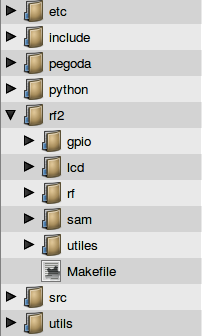
\includegraphics[scale=.4]{Imagenes/estructura_librfid.png} 
  \end{center}
  \caption{Estructura de árbol de aplicación RF$^{2}$}\label{est_RF2} 
\end{figure}

gpio incluye fuentes para el manejo de los GPIO.

lcd incluye fuentes para el manejo del display.

rf incluye fuentes con funciones extra de utilidad para el manejo del lector/escritor RFID diseñado.

sam incluye los fuentes para la comunicación con la tarjeta de contacto.

utiles incluye fuentes con funciones útiles de la aplicación.

\bigskip
Dentro de cada uno de estos directorios se encuentra un archivo Makefile con las reglas de compilación correspondientes a cada uno.

\bigskip
Las modificaciones a los archivos de construcción de la aplicación para que contemplen el agregado del directorio rf2, como la creación de nuevas reglas para la construcción dentro de éste, se detallan a continuación.

\bigskip
Antes que nada se decidió modificar los archivos Makefile.am para que sepan de la existencia del nuevo directorio. Se modifican estos archivos debido a que nunca son borrados. Por ejemplo, si los cambios se hacen sobre los Makefile.in, puede pasar que en algún momento se regeneren borrando los cambios que se hicieron. Además, luego de entender la estructura y funcionamiento de estos archivos, es más fácil incluir una modificación en Makefile.am que en un Makefile.in o Makefile directamente.

Dentro del directorio utiles, se creó el archivo Variables\_Make que establece el valor de algunas variables específicas de la aplicación RF$^{2}$ como ser CC\_arm que hace referencia al gcc asociado con la herramienta de crosscompilación para ARM. 

\bigskip
Makefile.flags.am:
Aquí se indicó que se agregue rf2 a la ruta de búsqueda de archivos encabezados.

\begin{verbatim}
INCLUDES = \$(all_includes) -I$(top_srcdir)/include 
-I\$(top_srcdir)/rf2
\end{verbatim}

Makefile.am en el raíz:

\begin{verbatim}
include rf2/utiles/Variables_Make
\end{verbatim}
Con esto se aseguró que el resto de los subdirectorios pertenecientes a la librfid, sepan los valores de las variables específicas de la aplicación RF$^{2}$.

\bigskip
Luego se incluye el directorio rf2 a la aplicación, teniendo en cuenta que solo se va a incluir cuando se use un lector/escritor RFID con interfaz SPI.
\begin{verbatim}
if ENABLE_SPIDEV 
SUBDIRS += rf2 
endif
\end{verbatim}

Makefile.am en utils:
Este es el cambio más dificil de entender y surge de la observación (prueba y error) del archivo Makefile.in generado en cada ocasión que se utilizó la herramienta automake. Como la aplicación RF$^{2}$ se basa en la modificación de los fuentes de la herramienta librfid-tool, se deben agregar todas las dependencias con archivos del nuevo subdirectorio rf2.

\begin{verbatim}
librfid_tool_SOURCES = librfid-tool.c librfid-tool.h 
common.c common.h ../rf2/gpio/gpio.c ../rf2/gpio/gpio.h 
../rf2/rf/rc632_utils.c ../rf2/rf/rc632_utils.h 
../rf2/lcd/lcd16x2.c ../rf2/lcd/lcd16x2.h ../rf2/sam/sam.c 
../rf2/sam/sam.h ../rf2/sam/sam_util.c ../rf2/sam/sam_util.h 
../rf2/utiles/utiles.c ../rf2/utiles/utiles.h
\end{verbatim}

Cada .h y .c se traduce en un .o al crear el Makefile.in.

\newpage
Otro cambio necesario, ya que si no se incluye provoca errores de compilación, es el siguiente.

\begin{verbatim}
mifare_tool_SOURCES = mifare-tool.c common.c 
../rf2/gpio/gpio.c ../rf2/rf/rc632_utils.c 
../rf2/lcd/lcd16x2.c ../rf2/sam/sam.c 
../rf2/sam/sam_util.c ../rf2/utiles/utiles.c
\end{verbatim}

mifare-tool es otra herramienta de la librfid.

\bigskip
Luego se creó dentro del directorio rf2 un archivo Makefile que es el que ordena la construcción de todos los objetivos dentro de cada subdirectorio.

\begin{verbatim}
include utiles/Variables_Make 

all: gpio/gpio.o rf/rc632_utils.o lcd/lcd16x2.o 
sam/sam.o utiles/utiles.o 

gpio/gpio.o: 
	$(MAKE) -C gpio 

rf/rc632_utils.o: 
	$(MAKE) -C rf 

lcd/lcd16x2.o: 
	$(MAKE) -C lcd 

sam/sam.o: 
	$(MAKE) -C sam 
	 
utiles/utiles.o: 
	$(MAKE) -C utiles 

install: 

clean: 
	rm -f *.o 
	$(MAKE) -C gpio clean 
	$(MAKE) -C rf clean 
	$(MAKE) -C lcd clean 
	$(MAKE) -C sam clean 
	$(MAKE) -C utiles clean 

distclean: clean
\end{verbatim}

\bigskip
En este caso \$(MAKE) -C “directorio” indica que la regla de construcción del objetivo se encuentra en “directorio”.

\section{Crosscompilación de la aplicación final}\label{crosap}

Para guardar el resultado de la crosscompilación se creó un directorio work en el home del usuario.

\bigskip
\begin{verbatim}
$ ./autogen.sh
\end{verbatim}

Este paso es necesario siempre que se modifiquen los Makefile.am, en otro caso no. Se recuerda que este script genera los archivos Makefile.in y configure.

\bigskip
\begin{verbatim}
$ ./configure --enable-spidev --host=arm-angstrom-linux-gnueabi 
--prefix=/home/proyecto/work
\end{verbatim}

\bigskip
Se configura el sistema para lectores/escritores RFID con interfaz SPI, se indica la arquitectura de la SBC para la cual se compila y se indica el directorio donde se instala la aplicación. Luego de hecho esto ya no es necesario volver a ejecutarlo ya que los Makefile quedan creados con esta configuración.

\bigskip
\begin{verbatim}
$ make -j5 && make install
\end{verbatim}

Se construye la aplicación.

\bigskip
En el directorio work se encuentran cuatro nuevos directorios creados:

\bigskip
bin: incluye los binarios construidos.

include: directorio con los .h necesarios para correr la aplicación.

lib: la biblioteca en sí.

share: nada de utilidad.

\bigskip
El paso siguiente es copiar estos directorios en el sistema de archivos de la SBC.

\bigskip
Copia de archivos a la SBC:

\bigskip
Para realizar la copia conviene comprimir el resultado de la crosscompilación y luego enviarlo a la SBC.

\begin{verbatim}
$ tar -czf rf2.tar.gz bin include lib share
\end{verbatim}

\bigskip
Luego de enviar el archivo comprimido, es necesaria la copia de estos directorios en el sistema de archivos de la SBC.

\bigskip
Instalación en la SBC:

\begin{verbatim}
$ tar -xf rf2.tar.gz -C /usr
\end{verbatim}

Esto descomprime los directorios creados anteriormente, dentro del directorio /usr.

\bigskip
Se ejecuta la aplicación RF$^{2}$:

\begin{verbatim}
$ librfid-tool -n
\end{verbatim}


\section{Pruebas sobre las interfaces}

\subsection{led.c}\label{anx_sw_led}

\begin{verbatim}
#include <string.h>
#include <stdio.h>
#include <stdlib.h>
#include <unistd.h>
FILE *fp;

int main(int argc, char** argv)
{
  printf("\n**********************************\n"
  "* Welcome to PIN Blink program *\n"
  "* ....blinking pin 13 on expansion port *\n"
  "* ....rate of 1 Hz............ *\n"
  "**********************************\n");
  //create a variable to store whether we are 
  //sending a '1' or a '0'
  char set_value[4];
  //Integer to keep track of whether we want on or off
  int toggle = 0;
  //Using sysfs we need to write "134" 
  //to /sys/class/gpio/export
  //This will create the folder /sys/class/gpio/gpio134
  if ((fp = fopen("/sys/class/gpio/export", "ab")) == NULL)
  {
    printf("Cannot open export file.\n");
    exit(1);
  }
  //Set pointer to begining of the file
  rewind(fp);
  //Write our value of "134" to the file
  strcpy(set_value,"134");
  fwrite(&set_value, sizeof(char), 3, fp);
  fclose(fp);
  printf("...export file accessed, new pin now accessible\n");
  //SET DIRECTION
  //Open the LED's sysfs file in binary for 
  //reading and writing, store file pointer in fp
  if ((fp = fopen("/sys/class/gpio/gpio134/direction", "rb+")) 
  == NULL)
  {
    printf("Cannot open direction file.\n");
    exit(1);
  }
  //Set pointer to begining of the file
  rewind(fp);
  //Write our value of "out" to the file
  strcpy(set_value,"out");
  fwrite(&set_value, sizeof(char), 3, fp);
  fclose(fp);
  printf("...direction set to output\n");
  //SET VALUE
  //Open the LED's sysfs file in binary for 
  //reading and writing, store file pointer in fp
  if ((fp = fopen("/sys/class/gpio/gpio134/value", "rb+")) 
  == NULL)
  {
    printf("Cannot open value file.\n");
    exit(1);
  }
  //Set pointer to begining of the file
  rewind(fp);
  //Write our value of "1" to the file
  strcpy(set_value,"1");
  fwrite(&set_value, sizeof(char), 1, fp);
  fclose(fp);
  printf("...value set to 1...\n");
  //Run an infinite loop - will require 
  //Ctrl-C to exit this program
  while(1)
  {
    //Set it so we know the starting value 
    //in case something above doesn't leave it as 1
    strcpy(set_value,"1");
    if ((fp = fopen("/sys/class/gpio/gpio134/value", "rb+")) 
    == NULL)
    {
      printf("Cannot open value file.\n");
      exit(1);
    }
    toggle = !toggle;
    if(toggle)
    {
      //Set pointer to begining of the file
      rewind(fp);
      //Write our value of "1" to the file
      strcpy(set_value,"1");
      fwrite(&set_value, sizeof(char), 1, fp);
      fclose(fp);
      printf("...value set to 1...\n");
    }
    else
    {
      //Set pointer to begining of the file
      rewind(fp);
      //Write our value of "0" to the file
      strcpy(set_value,"0");
      fwrite(&set_value, sizeof(char), 1, fp);
      fclose(fp);
      printf("...value set to 0...\n");
    }
    //Pause for one second
    sleep(1);
  }
  return 0;
}
\end{verbatim}



\subsection{uart.c}\label{anx_sw_uart}

\begin{verbatim}
#include <sys/types.h>
#include <sys/stat.h>
#include <fcntl.h>
#include <termios.h>
#include <stdio.h>

#define BAUDRATE B9600
#define SERIALPORT "/dev/ttyS1"
#define _POSIX_SOURCE 1 /* POSIX compliant source */
#define FALSE 0
#define TRUE 1
#define BUFFWRITE 10
#define BUFFREAD 255

int fd; //descriptor del archivo asociado con tty
struct termios oldtio,newtio;

//inicialización
int tty_init (void)
{
  //abrimos el puerto ttyS1
  fd = open(SERIALPORT, O_RDWR | O_NOCTTY ); 
  if(fd<0)
  return 0; //hubo errores
  else
  {
    printf("Puerto %s, abierto. fd: %d\n", SERIALPORT, fd);
    /* save current port settings */
    tcgetattr(fd,&oldtio); 
    //bzero(&newtio, sizeof(newtio));
    newtio.c_cflag = BAUDRATE | CS8 | CLOCAL | CREAD;
    newtio.c_iflag = IGNPAR;
    newtio.c_oflag = 0;
    /* set input mode (non-canonical, no echo,...) */
    newtio.c_lflag = 0;
    /* inter-character timer unused */
    newtio.c_cc[VTIME] = 0;
    /* bloqueo la lectura hasta que llegue 1 caracter */ 
    newtio.c_cc[VMIN] = 1; 
    tcflush(fd, TCIFLUSH);
    tcsetattr(fd,TCSANOW,&newtio);
    return 1; //no hubo errores
  }
}

//envio de un caracter por UART
void escribir (char s[10])
{
  write(fd, s, BUFFWRITE); //escribe el string en UART-Tx
  printf("dato enviado: %s\n", s);
}

//lectura de caracter por UART
char leer (void)
{
  char r[BUFFREAD];
  if(read(fd, r, BUFFREAD) == -1)
  return 0; //No hay datos o se incluyen ceros
  else
  return r[0]; //no hubo errores, se retorna el valor leido
}

int main (void)
{
  //cantidad de caracteres leidos por UART
  int UART_get_return; 
  //indica si se pudo abrir el puerto o no
  int UART_init_return; 
  char buff[BUFFREAD];
  //inicializacion de la UART
  UART_init_return = tty_init(); 
  
  //no se pudo abrir el puerto
  if (UART_init_return == 0) 
  printf("no se pudo abrir el puerto ttyS1.\n");
  else //se pudo abrir el puerto
  {
    char str[10]={'a','s','d','f','g','h','j','k','l','t'};
    escribir(str);
    UART_get_return = read(fd,buff,BUFFREAD);
    
    // 0 = no se encontraron datos en Rx
    if (UART_get_return == 0) 
    printf("no hay datos para leer\n");
    else //1 = dato encontrado
    {
      buff[UART_get_return]=0;
      printf("dato leido: %s:%d\n", buff,UART_get_return);
    }
  }
  tcsetattr(fd,TCSANOW,&oldtio);
}

\end{verbatim}

\section{Licencias y versiones de las bibliotecas y herramientas open-source empleadas}

\begin{itemize}
\item librfid: licencia GNU GPL V2, versión 0.2.0.
\item PCSC-Lite: licencia BSD, versión 1.7.4.
\item CT/API: licencia GPL, versión 1.1.
\item lcd: licencia GNU LGPL, versión 1.1.
\item GPIO: licencia GNU LGPL, versión 1.0.
\item OpenEmbedded: licencia GPL/MIT, versión 2011.03.
\item Bitbake: licencia GPL/MIT, versión 1.10.2.
\item KiCad: licencia GPL, versión 2010-05-05.
\item gEDA: licencia GNU GPL V2, versión 20091103.
\end{itemize}